% paper-to-book template (filled in by pipeline/p2b.py build)
\documentclass[11pt,letterpaper,openright]{book}
\usepackage{p2bbook}
\begin{document}
\frontmatter
\begin{titlepage}\centering
\vspace*{2in}{\Huge Windmills: A Prerequisite Book\par}\vspace{0.4in}
{\Large A prerequisite book for Windmills of the minds: an algorithm for Fermat's Two Squares Theorem\par}\vspace{0.2in}{\large Hing Lun Chan\par}
\vfill{\small Assumed background: arithmetic (addition, subtraction, multiplication); high-school algebra; basic proof writing (induction, contradiction); sets and functions\par}
\vspace{0.3in}{\footnotesize Built with paper-to-book. Every definition and theorem is tagged in the margin
with its source; quotations are checked automatically against the retrieved sources, and
statements marked \textsf{Lean \checkmk} are verified against Lean's mathlib.\par}
\end{titlepage}
\tableofcontents
\chapter*{How to read this book}\addcontentsline{toc}{chapter}{How to read this book}
The chapters build, in order, everything the paper uses that goes beyond the assumed background.
Each definition, theorem and quotation, and each paragraph that cites a source, begins with a
small grey number in brackets, such as \textcolor{srcgray}{\footnotesize[1]}, referring to the note
with the same number at the foot of the page. The note says where it comes from. These numbers
are never part of the mathematics; they always stand in front of what they refer to, set apart by
a space. The notes may say:
\begin{itemize}
\item \srcok{source}{§} --- quoted from a retrieved source, and the quotation was checked automatically;
\item \leanok{name} --- the statement matches a declaration in Lean's mathlib that compiles;
\item \leanpending{name} --- a formal counterpart exists but has not been checked yet;
\item \derivedtag{sources} --- not stated in any source, but proved in this book from the sourced results named, with the proof given and checked in Lean;
\item \unsourced{} or \srcbad{id} --- not backed by a checked source: treat with suspicion.
\end{itemize}
Shaded boxes are definitions; passages with a grey bar on the left are verbatim quotations;
blue boxes show where the idea appears in the paper. The last part is the paper itself.
\mainmatter
% 01-whole-numbers.md: generated from books/windmills/chapters/01-whole-numbers.md; edit freely.
\hypertarget{whole-numbers}{%
\chapter{Whole Numbers}\label{whole-numbers}}

The paper proves a theorem of Fermat about primes and squares, and turns
the proof into an algorithm. In the paper's own words:

\bpush\begin{bquote}

\srcnote{\srcok{paper}{§1}{C1-16}}Fermat's two squares theorem, dated
back to 1640, states that a prime \(n\) that is one more than a multiple
of \(4\) can be uniquely expressed as a sum of odd and even squares

\end{bquote}\bpop

To follow it you need five ideas about whole numbers: when one number
\emph{divides} another, \emph{division with remainder}, \emph{even and
odd}, \emph{primes}, and \emph{squares}. This chapter introduces each
and proves the few facts about them that the paper uses.

Throughout, a \emph{number} means a natural number
\(0, 1, 2, 3, \dots\), as in the paper:

\bpush\begin{bquote}

\srcnote{\srcok{paper}{§1.3}{C1-18}}The set of natural numbers is
denoted by \(\mathbb{N}\), counting from \(0\)

\end{bquote}\bpop

Some of the definitions quoted below are stated for all integers,
negative ones included; we only ever apply them to natural numbers.

\hypertarget{divisibility}{%
\section{Divisibility}\label{divisibility}}

\bpush\begin{bdefinition}\label{def-divides}\srcnote{\srcok{wp-divisor}{Definition}{L001} \enspace\textperiodcentered\enspace \leanok{Dvd.dvd}}

\index{divisible}

A number \(m\) is \textbf{divisible} by a nonzero number \(d\) if
\(m = kd\) for some number \(k\). We then say \(d\) \emph{divides}
\(m\), and write \(d \mid m\).

\end{bdefinition}\bpop

\bpush\begin{bquote}

\srcnote{\srcok{wp-divisor}{Definition}{L001}}An integer n is divisible
by a nonzero integer m if there exists an integer k such that n = k m .

\end{bquote}\bpop

So \(3 \mid 12\) because \(12 = 4 \cdot 3\), but \(3 \nmid 13\): no
number \(k\) has \(3k = 13\). Every number \(m \geq 1\) is divisible by
\(1\) and by itself, since \(m = m \cdot 1\). These two are its
\emph{trivial} divisors:

\bpush\begin{bquote}

\srcnote{\srcok{wp-divisor}{Terminology}{C1-01}}1, −1, n and − n are
known as the trivial divisors of n

\end{bquote}\bpop

\srccitenote{\srccite{wp-divisor}{Terminology}}A number greater than
\(1\) with a divisor other than these is called \emph{composite}.

\bpush\begin{bremark}

The paper writes \(n \mid m\) for ``\(n\) divides \(m\)'', with \(n\) as
the divisor, and from here on we use its letters (§1.3):

\bpush\begin{bquote}

\srcnote{\srcok{paper}{§1.3}{C1-17}}We write
\HOLinline{\HOLFreeVar{n}\;\HOLConst{\ensuremath{\mid}}\;\HOLFreeVar{m}}
when \(n\) divides \(m\), which is equivalent to
\HOLinline{\HOLFreeVar{m}\;\ensuremath{\equiv}\;\HOLNumLit{0}\;\ensuremath{(}\ensuremath{\bmod}\;\HOLFreeVar{n}\ensuremath{)}}
when
\HOLinline{\HOLFreeVar{n}\;\HOLSymConst{\HOLTokenNotEqual{}}\;\HOLNumLit{0}}.

\end{bquote}\bpop

Lean's mathlib, which checks the statements in this book, defines
\(d \mid m\) for every \(d\), including \(d = 0\): there \(0 \mid m\)
holds only when \(m = 0\). For \(d \ne 0\) the two definitions agree.

\end{bremark}\bpop

\hypertarget{division-with-remainder}{%
\section{Division with remainder}\label{division-with-remainder}}

Most numbers don't divide each other exactly; what is left over is the
\emph{remainder}.

\bpush\begin{btheorem}\label{thm-division}\srcnote{\srcok{wp-euclidean-division}{Division theorem}{L002} \enspace\textperiodcentered\enspace \leanok{Book.Windmills.Ch01.division}; \leanok{Book.Windmills.Ch01.division_unique}}

\textbf{Division with remainder.} Given numbers \(m\) and \(n\) with
\(n \neq 0\), there are unique numbers \(q\) (the \emph{quotient}) and
\(r\) (the \emph{remainder}) such that
\[m = nq + r \qquad\text{and}\qquad 0 \le r < n.\]

\end{btheorem}\bpop

\bpush\begin{bquote}

\srcnote{\srcok{wp-euclidean-division}{Division theorem}{L002}}Given two
integers a and b , with b ≠ 0 , there exist unique integers q and r such
that a = b q + r , and 0 ≤ r \textless{} \textbar{} b \textbar{}

\end{bquote}\bpop

\bpush\begin{bexample}

\srccitenote{\srccite{wp-euclidean-division}{Intuitive example}}Dividing
\(17\) by \(3\): the quotient is \(5\) and the remainder is \(2\), since
\(17 = 3 \cdot 5 + 2\) and \(2 < 3\).

\end{bexample}\bpop

\bpush\begin{proof}

\emph{Existence.} Start with \(r = m\) and \(q = 0\), so that
\(m = nq + r\). While \(r \ge n\), replace \(r\) by \(r - n\) and \(q\)
by \(q + 1\); the equation \(m = nq + r\) still holds. Each step makes
\(r\) smaller, and a number can only get smaller finitely many times, so
the process stops, with \(r < n\).

\emph{Uniqueness.} Suppose also \(m = nq' + r'\) with \(r' < n\), and
say \(r \le r'\) (otherwise swap the two). Then \(nq = nq' + (r' - r)\),
so \(q \ge q'\) and \(r' - r = n(q - q')\). The left side is less than
\(n\), and the only multiple of \(n\) less than \(n\) is \(0\). So
\(r' = r\), and then \(q' = q\).

\end{proof}\bpop

The paper writes the quotient as \(m \operatorname{div} n\) and the
remainder as \(m \operatorname{mod} n\):

\bpush\begin{bquote}

\srcnote{\srcok{paper}{§1.3}{C1-05}}The integer quotient and remainder
of \(m\) divided by \(n\) are written as
\HOLinline{\HOLFreeVar{m}\;\HOLConst{\HOLConst{div}}\;\HOLFreeVar{n}}
and
\HOLinline{\HOLFreeVar{m}\;\HOLConst{\HOLConst{mod}}\;\HOLFreeVar{n}},
respectively.

\end{bquote}\bpop

For example, \(17 \operatorname{div} 3 = 5\) and
\(17 \operatorname{mod} 3 = 2\). Dividing leaves nothing over exactly
when \(n\) divides \(m\):

\bpush\begin{bproposition}\label{prop-dvd-mod}\srcnote{\derivedtag{\texttt{wp-divisor}, \texttt{wp-euclidean-division}} \enspace\textperiodcentered\enspace \leanok{Book.Windmills.Ch01.dvd_iff_mod}}

For \(n \ne 0\): \(\ n \mid m\) if and only if
\(m \operatorname{mod} n = 0\).

\end{bproposition}\bpop

\bpush\begin{proof}

If \(m = kn\), then \(m = nk + 0\) with \(0 < n\), so by uniqueness the
remainder is \(0\). Conversely, if the remainder is \(0\), then
\(m = nq\), so \(n \mid m\).

\end{proof}\bpop

\hypertarget{even-and-odd}{%
\section{Even and odd}\label{even-and-odd}}

\bpush\begin{bdefinition}\label{def-parity}\srcnote{\srcok{wp-parity}{Definition}{C1-06}; \srcok{wp-parity}{lead}{C1-20} \enspace\textperiodcentered\enspace \leanok{Even}; \leanok{Odd}}

\index{even}

A number is \textbf{even} if it has the form \(2k\), and \textbf{odd} if
it has the form \(2k + 1\), for some number \(k\). Whether a number is
even or odd is called its \textbf{parity}.

\end{bdefinition}\bpop

\bpush\begin{bquote}

\srcnote{\srcok{wp-parity}{Definition}{C1-06}}An even number is an
integer of the form x = 2 k where k is an integer; {[} 4 {]} an odd
number is an integer of the form x = 2 k + 1

\end{bquote}\bpop

\bpush\begin{bquote}

\srcnote{\srcok{wp-parity}{lead}{C1-20}}parity is the property of an
integer of whether it is even or odd

\end{bquote}\bpop

\bpush\begin{btheorem}\label{thm-even-odd}\srcnote{\derivedtag{\texttt{wp-euclidean-division}, \texttt{wp-parity}} \enspace\textperiodcentered\enspace \leanok{Book.Windmills.Ch01.even_or_odd}; \leanok{Book.Windmills.Ch01.not_even_and_odd}; \leanok{Book.Windmills.Ch01.even_iff_mod}; \leanok{Book.Windmills.Ch01.odd_iff_mod}}

Every number is either even or odd, and not both. A number \(n\) is even
exactly when \(n \operatorname{mod} 2 = 0\), and odd exactly when
\(n \operatorname{mod} 2 = 1\).

\end{btheorem}\bpop

\bpush\begin{proof}

Divide \(n\) by \(2\): \(n = 2q + r\) with \(r \in \{0, 1\}\). If
\(r = 0\) then \(n = 2q\) is even; if \(r = 1\) then \(n = 2q + 1\) is
odd. So every number is one or the other.

Conversely, if \(n = 2k\) then \(n = 2k + 0\), and if \(n = 2k + 1\)
then that is already a division by \(2\) with remainder \(1\). By
uniqueness of the remainder, an even number has remainder \(0\) and an
odd number has remainder \(1\); in particular no number is both.

\end{proof}\bpop

Parity behaves simply under addition: even \(+\) even and odd \(+\) odd
are even, while even \(+\) odd is odd (write the numbers as \(2a\) or
\(2a + 1\) and add). Parity matters throughout the paper, both of
numbers and, from Chapter 5 on, of the \emph{sizes of sets}:

\bpush\begin{bquote}

\srcnote{\srcok{paper}{Abstract}{C1-19}}The theory behind involves
involutions on a finite set, especially the parity of the number of
fixed points in the involutions.

\end{bquote}\bpop

\bpush\begin{bremark}

mathlib phrases these definitions slightly differently: \texttt{Even\ n}
says \(n = r + r\) for some \(r\), and \texttt{Odd\ n} says
\(n = 2k + 1\). The first is the same as \(n = 2r\).

\end{bremark}\bpop

\bpush\begin{binpaper}

The paper's notation section (§1.3) writes \(\mathsf{even}\ n\) and
\(\mathsf{odd}\ n\) for these two properties:

\bpush\begin{bquote}

\srcnote{\srcok{paper}{§1.3}{C1-08}}prime n means it is a prime, and
even n or odd n denotes its parity

\end{bquote}\bpop

\end{binpaper}\bpop

\hypertarget{prime-numbers}{%
\section{Prime numbers}\label{prime-numbers}}

\bpush\begin{bdefinition}\label{def-prime}\srcnote{\srcok{wp-prime}{lead}{L005} \enspace\textperiodcentered\enspace \leanok{Nat.Prime}}

\index{prime number}

A \textbf{prime number} is a number greater than \(1\) that is not a
product of two smaller numbers.

\end{bdefinition}\bpop

\bpush\begin{bquote}

\srcnote{\srcok{wp-prime}{lead}{L005}}A prime number (or a prime ) is a
natural number greater than 1 that is not a product of two smaller
natural numbers.

\end{bquote}\bpop

\srccitenote{\srccite{wp-prime}{Definition and examples}}The
\emph{divisors} of \(n\) are the numbers that divide it evenly. Primes
are exactly the numbers greater than \(1\) with no divisors except the
trivial ones:

\bpush\begin{bproposition}\label{prop-prime-divisors}\srcnote{\srcok{wp-prime}{Definition and examples}{C1-09} \enspace\textperiodcentered\enspace \leanok{Nat.prime_def}}

A number \(p\) is prime if and only if it has exactly two positive
divisors, \(1\) and \(p\) (so in particular \(p \ge 2\)).

\end{bproposition}\bpop

\bpush\begin{proof}

First, \(0\) and \(1\) are not prime (the definition needs \(p > 1\)),
and neither has exactly the two positive divisors \(1\) and \(p\): every
positive number divides \(0\), and \(1\) has the single positive divisor
\(1\). So take \(p > 1\).

If \(p\) is a product \(ab\) of two numbers smaller than \(p\), then
\(a \ne 1\) (else \(b = p\), which is not smaller) and \(a \ne p\), so
\(a\) is a positive divisor other than \(1\) and \(p\).

Conversely, suppose \(p\) has a positive divisor \(a\) other than \(1\)
and \(p\), say \(p = ab\). Then \(b \ge 1\) (as \(p \ne 0\)), so
\(a \le p\); since \(a \ne p\) and \(a \ne 1\), we have \(1 < a < p\).
Then \(b = p / a\) satisfies \(1 < b < p\) as well, so \(p\) is a
product of two smaller numbers.

\end{proof}\bpop

In the same way, a number greater than \(1\) is composite exactly when
it is not prime.

\bpush\begin{bexample}

\srccitenote{\srccite{wp-prime}{Definition and examples}}\(7\) is prime:
none of \(2, 3, 4, 5, 6\) divides it. The primes below \(30\) are
\(2, 3, 5, 7, 11, 13, 17, 19, 23, 29\).

\end{bexample}\bpop

Two facts about primes matter for the paper.

\bpush\begin{btheorem}\label{thm-only-even-prime}\srcnote{\srcok{paper}{§2}{C1-12} \enspace\textperiodcentered\enspace \leanok{Book.Windmills.Ch01.prime_even_eq_two}}

The only even prime is \(2\).

\end{btheorem}\bpop

\bpush\begin{bquote}

\srcnote{\srcok{paper}{§2}{C1-12}}The only even prime is
\HOLinline{\HOLNumLit{2}\;\HOLSymConst{=}\;\HOLNumLit{1}\ensuremath{{\sp{\HOLNumLit{2}}}}\;\HOLSymConst{\ensuremath{+}}\;\HOLNumLit{1}\ensuremath{{\sp{\HOLNumLit{2}}}}},
a sum of two squares.

\end{bquote}\bpop

\bpush\begin{proof}

An even number \(n\) has \(2 \mid n\). If \(n\) is prime, its only
divisors are \(1\) and \(n\), so \(n = 2\).

\end{proof}\bpop

\bpush\begin{btheorem}\label{thm-odd-prime-mod-4}\srcnote{\srcok{paper}{§2}{C1-13} \enspace\textperiodcentered\enspace \leanok{Book.Windmills.Ch01.odd_prime_mod_four}}

An odd prime leaves a remainder of \(1\) or \(3\) when divided by \(4\).

\end{btheorem}\bpop

\bpush\begin{proof}

Divide the prime \(p\) by \(4\): \(p = 4q + r\) with
\(r \in \{0, 1, 2, 3\}\). If \(r\) were \(0\) or \(2\), then
\(p = 2(2q)\) or \(p = 2(2q + 1)\) would be even. Since \(p\) is odd,
\(r\) is \(1\) or \(3\).

\end{proof}\bpop

So the odd primes fall into two families: those of the form \(4k + 1\)
(\(5, 13, 17, 29, \dots\)) and those of the form \(4k + 3\)
(\(3, 7, 11, 19, 23, \dots\)). The paper's theorem is about the first
family.

\bpush\begin{binpaper}

§2 opens with exactly these two facts: the only even prime is a sum of
two squares, and the odd primes split by their remainder on division by
\(4\).

\end{binpaper}\bpop

\hypertarget{squares}{%
\section{Squares}\label{squares}}

\bpush\begin{bdefinition}\label{def-square}\srcnote{\srcok{wp-square-number}{lead}{L006} \enspace\textperiodcentered\enspace \leanok{IsSquare}}

\index{square number}

A \textbf{square number} (or perfect square) is the square
\(k^2 = k \cdot k\) of a number \(k\).

\end{bdefinition}\bpop

\bpush\begin{bquote}

\srcnote{\srcok{wp-square-number}{lead}{L006}}a square number or perfect
square is an integer that is the square of an integer

\end{bquote}\bpop

The first few are \(0, 1, 4, 9, 16, 25, 36, 49, 64\). A \emph{sum of two
squares} is a number of the form \(u^2 + v^2\); for instance
\(13 = 3^2 + 2^2\) and \(29 = 5^2 + 2^2\), while no choice of \(u, v\)
gives \(3\), \(7\) or \(11\) (the squares up to \(11\) are only
\(0, 1, 4, 9\), and no two of them add up to \(3\), \(7\) or \(11\)).
Chapter 2 explains why.

\bpush\begin{binpaper}

The paper writes \(\mathsf{square}\ n\) for ``\(n\) is a square''
(§1.3):

\bpush\begin{bquote}

\srcnote{\srcok{paper}{§1.3}{C1-15}}For a natural number
\(n \in \mathbb{N}\), \HOLinline{\HOLConst{square}\;\HOLFreeVar{n}}
means it is a square:
\HOLinline{\HOLSymConst{\HOLTokenExists{}}\HOLBoundVar{k}.\;\HOLFreeVar{n}\;\HOLSymConst{=}\;\HOLBoundVar{k}\HOLSymConst{\ensuremath{\sp{2}}}}

\end{bquote}\bpop

\end{binpaper}\bpop

\hypertarget{exercises}{%
\section{Exercises}\label{exercises}}

\bpush\begin{bexercise}

Find the quotient and remainder when \(29\) is divided by \(4\), and
when \(61\) is divided by \(4\). Both are prime; which family of odd
primes does each belong to?

\end{bexercise}\bpop

\bpush\begin{bexercise}

Show that if \(n \mid a\) and \(n \mid b\) then \(n \mid a + b\).

\end{bexercise}\bpop

\bpush\begin{bexercise}

Show that the square of an odd number is odd. (Write the number as
\(2k + 1\).)

\end{bexercise}\bpop

\bpush\begin{bexercise}

Write each of \(5, 13, 17, 29, 37, 41\) as a sum of two squares.

\end{bexercise}\bpop

% The paper, with its reader's guide.
\part{The Paper}
\chapter*{Reader's guide to the paper}\addcontentsline{toc}{chapter}{Reader's guide to the paper}
The paper follows exactly as published, slightly reduced. Along the foot of each page are the concepts from this book that appear on it, with the chapter that teaches them. The first appearance of each:

\begin{longtable}{p{0.5\textwidth}ll}
Divisibility & Chapter~1 & p.~1 of the paper\\
Even and odd numbers & Chapter~1 & p.~1 of the paper\\
Prime numbers & Chapter~1 & p.~1 of the paper\\
Division with remainder & Chapter~1 & p.~2 of the paper\\
Square numbers & Chapter~1 & p.~2 of the paper\\
\end{longtable}
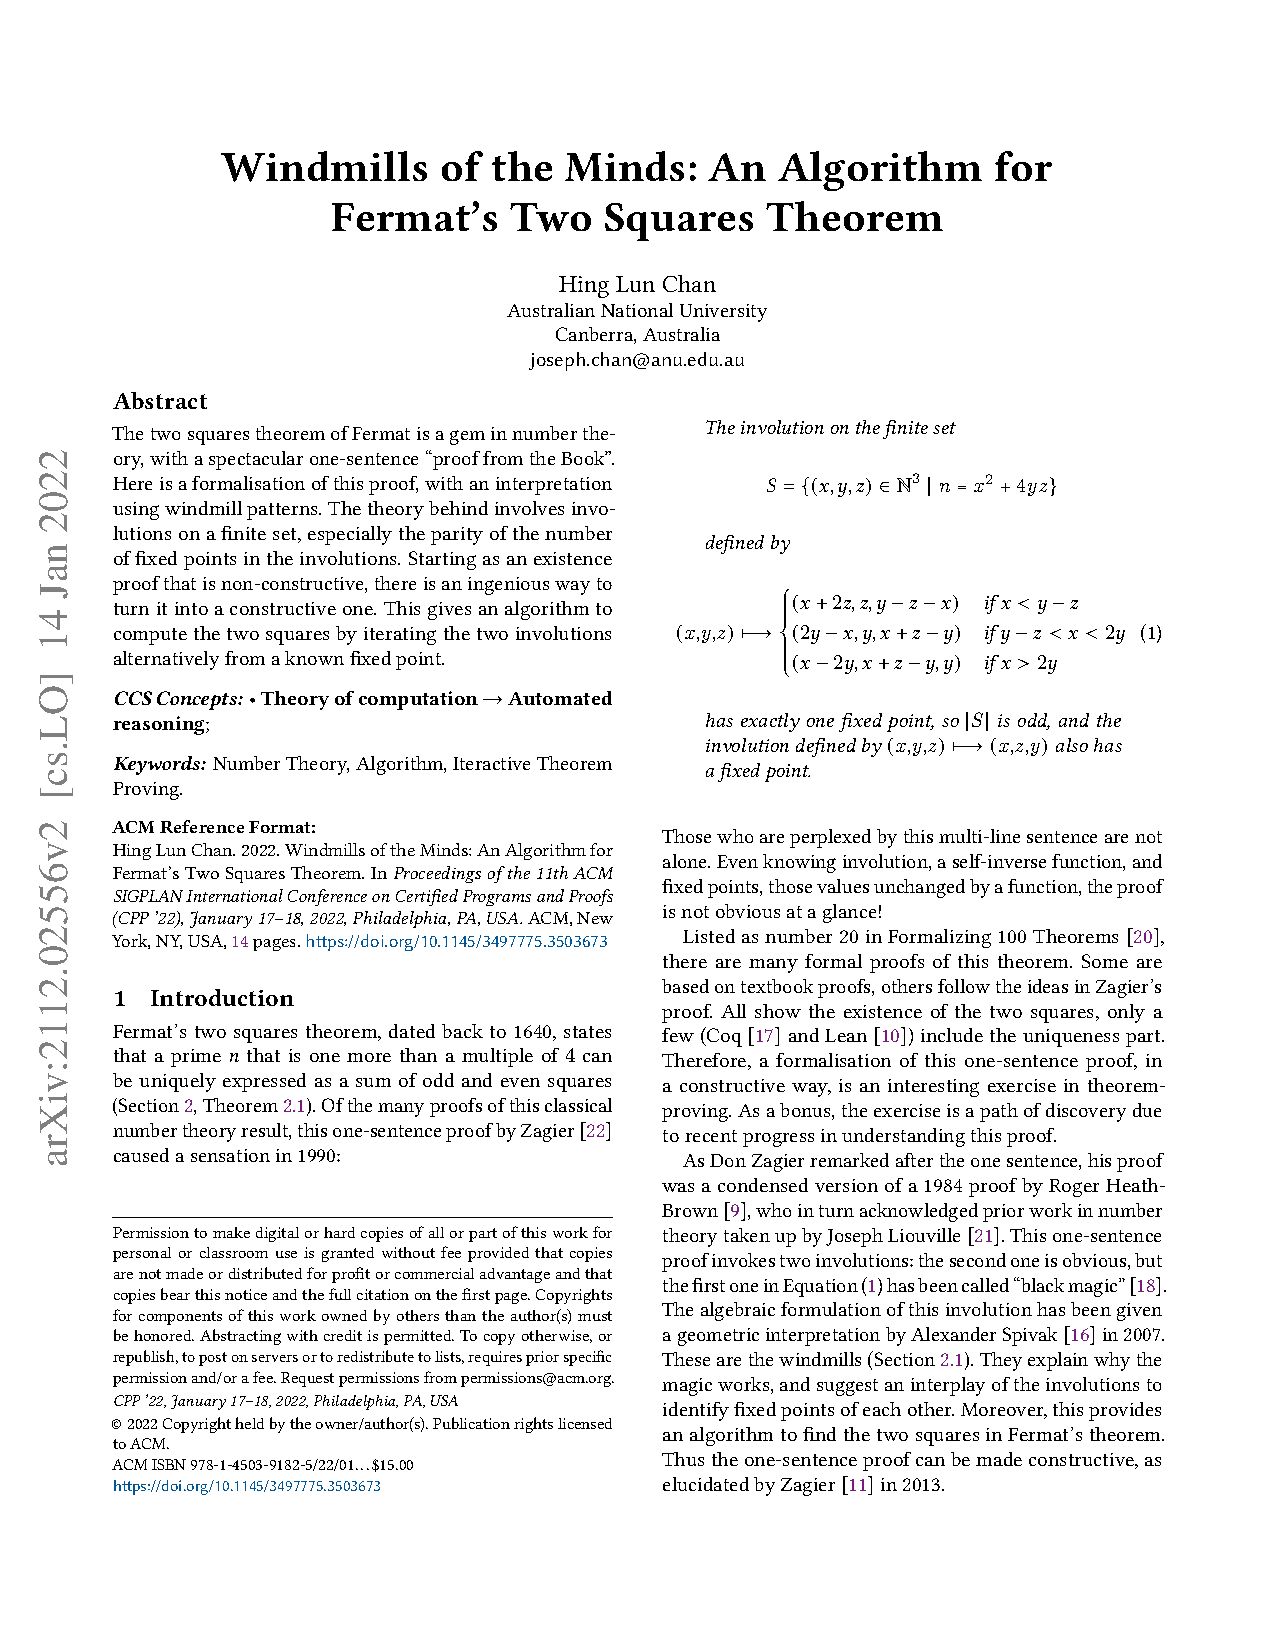
\includepdf[pages=1,scale=0.88,offset=0in 0.42in,pagecommand={\thispagestyle{empty}\papernote{\textbf{In this book:} Divisibility (Ch.~1) \enspace\textperiodcentered\enspace Even and odd numbers (Ch.~1) \enspace\textperiodcentered\enspace Prime numbers (Ch.~1)}}]{paper.pdf}
\includepdf[pages=2,scale=0.88,offset=0in 0.42in,pagecommand={\thispagestyle{empty}\papernote{\textbf{In this book:} Division with remainder (Ch.~1) \enspace\textperiodcentered\enspace Even and odd numbers (Ch.~1) \enspace\textperiodcentered\enspace Prime numbers (Ch.~1) \enspace\textperiodcentered\enspace Square numbers (Ch.~1)}}]{paper.pdf}
\includepdf[pages=3,scale=0.88,offset=0in 0.42in,pagecommand={\thispagestyle{empty}\papernote{\textbf{In this book:} Division with remainder (Ch.~1) \enspace\textperiodcentered\enspace Even and odd numbers (Ch.~1) \enspace\textperiodcentered\enspace Prime numbers (Ch.~1) \enspace\textperiodcentered\enspace Square numbers (Ch.~1)}}]{paper.pdf}
\includepdf[pages=4,scale=0.88,offset=0in 0.42in,pagecommand={\thispagestyle{empty}\papernote{\textbf{In this book:} Prime numbers (Ch.~1) \enspace\textperiodcentered\enspace Square numbers (Ch.~1)}}]{paper.pdf}
\includepdf[pages=5,scale=0.88,offset=0in 0.42in,pagecommand={\thispagestyle{empty}\papernote{}}]{paper.pdf}
\includepdf[pages=6,scale=0.88,offset=0in 0.42in,pagecommand={\thispagestyle{empty}\papernote{}}]{paper.pdf}
\includepdf[pages=7,scale=0.88,offset=0in 0.42in,pagecommand={\thispagestyle{empty}\papernote{\textbf{In this book:} Division with remainder (Ch.~1) \enspace\textperiodcentered\enspace Even and odd numbers (Ch.~1) \enspace\textperiodcentered\enspace Prime numbers (Ch.~1) \enspace\textperiodcentered\enspace Square numbers (Ch.~1)}}]{paper.pdf}
\includepdf[pages=8,scale=0.88,offset=0in 0.42in,pagecommand={\thispagestyle{empty}\papernote{}}]{paper.pdf}
\includepdf[pages=9,scale=0.88,offset=0in 0.42in,pagecommand={\thispagestyle{empty}\papernote{\textbf{In this book:} Divisibility (Ch.~1) \enspace\textperiodcentered\enspace Division with remainder (Ch.~1) \enspace\textperiodcentered\enspace Even and odd numbers (Ch.~1)}}]{paper.pdf}
\includepdf[pages=10,scale=0.88,offset=0in 0.42in,pagecommand={\thispagestyle{empty}\papernote{\textbf{In this book:} Divisibility (Ch.~1) \enspace\textperiodcentered\enspace Division with remainder (Ch.~1) \enspace\textperiodcentered\enspace Even and odd numbers (Ch.~1)}}]{paper.pdf}
\includepdf[pages=11,scale=0.88,offset=0in 0.42in,pagecommand={\thispagestyle{empty}\papernote{\textbf{In this book:} Division with remainder (Ch.~1) \enspace\textperiodcentered\enspace Even and odd numbers (Ch.~1) \enspace\textperiodcentered\enspace Prime numbers (Ch.~1)}}]{paper.pdf}
\includepdf[pages=12,scale=0.88,offset=0in 0.42in,pagecommand={\thispagestyle{empty}\papernote{\textbf{In this book:} Division with remainder (Ch.~1) \enspace\textperiodcentered\enspace Even and odd numbers (Ch.~1) \enspace\textperiodcentered\enspace Prime numbers (Ch.~1) \enspace\textperiodcentered\enspace Square numbers (Ch.~1)}}]{paper.pdf}
\includepdf[pages=13,scale=0.88,offset=0in 0.42in,pagecommand={\thispagestyle{empty}\papernote{\textbf{In this book:} Prime numbers (Ch.~1)}}]{paper.pdf}
\includepdf[pages=14,scale=0.88,offset=0in 0.42in,pagecommand={\thispagestyle{empty}\papernote{\textbf{In this book:} Division with remainder (Ch.~1) \enspace\textperiodcentered\enspace Prime numbers (Ch.~1) \enspace\textperiodcentered\enspace Square numbers (Ch.~1)}}]{paper.pdf}
\backmatter
\chapter{Sources}
Every source used, as retrieved for this book. The identifiers in the margins refer to this list.
\begin{description}\item[\texttt{ml-function-basic}] https://leanprover-community.github.io/mathlib4\_docs/Mathlib/Logic/Function/Basic.html. \url{https://leanprover-community.github.io/mathlib4_docs/Mathlib/Logic/Function/Basic.html} --- 1 of 1 quotations verified (retrieved 2026-11-12).
\item[\texttt{ml-periodic}] https://leanprover-community.github.io/mathlib4\_docs/Mathlib/Dynamics/PeriodicPts/Defs.html. \url{https://leanprover-community.github.io/mathlib4_docs/Mathlib/Dynamics/PeriodicPts/Defs.html} --- 3 of 3 quotations verified (retrieved 2026-11-12).
\item[\texttt{paper}] Windmills of the minds: an algorithm for Fermat's Two Squares Theorem. \url{arXiv:2112.02556} --- 48 of 48 quotations verified (retrieved 2026-11-12).
\item[\texttt{wp-bijection}] https://en.wikipedia.org/wiki/Bijection. \url{https://en.wikipedia.org/wiki/Bijection} --- 1 of 1 quotations verified (retrieved 2026-11-12).
\item[\texttt{wp-cardinality}] https://en.wikipedia.org/wiki/Cardinality. \url{https://en.wikipedia.org/wiki/Cardinality} --- 2 of 2 quotations verified (retrieved 2026-11-12).
\item[\texttt{wp-cartesian}] https://en.wikipedia.org/wiki/Cartesian\_product. \url{https://en.wikipedia.org/wiki/Cartesian_product} --- 1 of 1 quotations verified (retrieved 2026-11-12).
\item[\texttt{wp-composition}] https://en.wikipedia.org/wiki/Function\_composition. \url{https://en.wikipedia.org/wiki/Function_composition} --- 1 of 1 quotations verified (retrieved 2026-11-12).
\item[\texttt{wp-divisor}] https://en.wikipedia.org/wiki/Divisor. \url{https://en.wikipedia.org/wiki/Divisor} --- 3 of 3 quotations verified (retrieved 2026-11-12).
\item[\texttt{wp-euclidean-division}] https://en.wikipedia.org/wiki/Euclidean\_division. \url{https://en.wikipedia.org/wiki/Euclidean_division} --- 3 of 3 quotations verified (retrieved 2026-11-12).
\item[\texttt{wp-fermat-two-squares}] https://en.wikipedia.org/wiki/Fermat\%27s\_theorem\_on\_sums\_of\_two\_squares. \url{https://en.wikipedia.org/wiki/Fermat%27s_theorem_on_sums_of_two_squares} --- 4 of 4 quotations verified (retrieved 2026-11-12).
\item[\texttt{wp-finite-set}] https://en.wikipedia.org/wiki/Finite\_set. \url{https://en.wikipedia.org/wiki/Finite_set} --- 1 of 1 quotations verified (retrieved 2026-11-12).
\item[\texttt{wp-fixed-point}] https://en.wikipedia.org/wiki/Fixed\_point\_(mathematics). \url{https://en.wikipedia.org/wiki/Fixed_point_(mathematics)} --- 1 of 1 quotations verified (retrieved 2026-11-12).
\item[\texttt{wp-hol}] https://en.wikipedia.org/wiki/HOL\_(proof\_assistant). \url{https://en.wikipedia.org/wiki/HOL_(proof_assistant)} --- 2 of 2 quotations verified (retrieved 2026-11-12).
\item[\texttt{wp-inverse}] https://en.wikipedia.org/wiki/Inverse\_function. \url{https://en.wikipedia.org/wiki/Inverse_function} --- 2 of 2 quotations verified (retrieved 2026-11-12).
\item[\texttt{wp-involution}] https://en.wikipedia.org/wiki/Involution\_(mathematics). \url{https://en.wikipedia.org/wiki/Involution_(mathematics)} --- 9 of 9 quotations verified (retrieved 2026-11-12).
\item[\texttt{wp-iterated}] https://en.wikipedia.org/wiki/Iterated\_function. \url{https://en.wikipedia.org/wiki/Iterated_function} --- 2 of 2 quotations verified (retrieved 2026-11-12).
\item[\texttt{wp-lambda}] https://en.wikipedia.org/wiki/Lambda\_calculus. \url{https://en.wikipedia.org/wiki/Lambda_calculus} --- 1 of 1 quotations verified (retrieved 2026-11-12).
\item[\texttt{wp-loop-invariant}] https://en.wikipedia.org/wiki/Loop\_invariant. \url{https://en.wikipedia.org/wiki/Loop_invariant} --- 2 of 2 quotations verified (retrieved 2026-11-12).
\item[\texttt{wp-modular}] https://en.wikipedia.org/wiki/Modular\_arithmetic. \url{https://en.wikipedia.org/wiki/Modular_arithmetic} --- 3 of 3 quotations verified (retrieved 2026-11-12).
\item[\texttt{wp-orbit}] https://en.wikipedia.org/wiki/Orbit\_(dynamics). \url{https://en.wikipedia.org/wiki/Orbit_(dynamics)} --- 1 of 1 quotations verified (retrieved 2026-11-12).
\item[\texttt{wp-parity}] https://en.wikipedia.org/wiki/Parity\_(mathematics). \url{https://en.wikipedia.org/wiki/Parity_(mathematics)} --- 5 of 5 quotations verified (retrieved 2026-11-12).
\item[\texttt{wp-periodic-point}] https://en.wikipedia.org/wiki/Periodic\_point. \url{https://en.wikipedia.org/wiki/Periodic_point} --- 3 of 3 quotations verified (retrieved 2026-11-12).
\item[\texttt{wp-permutation}] https://en.wikipedia.org/wiki/Permutation. \url{https://en.wikipedia.org/wiki/Permutation} --- 2 of 2 quotations verified (retrieved 2026-11-12).
\item[\texttt{wp-prime}] https://en.wikipedia.org/wiki/Prime\_number. \url{https://en.wikipedia.org/wiki/Prime_number} --- 4 of 4 quotations verified (retrieved 2026-11-12).
\item[\texttt{wp-proof-assistant}] https://en.wikipedia.org/wiki/Proof\_assistant. \url{https://en.wikipedia.org/wiki/Proof_assistant} --- 1 of 1 quotations verified (retrieved 2026-11-12).
\item[\texttt{wp-set-builder}] https://en.wikipedia.org/wiki/Set-builder\_notation. \url{https://en.wikipedia.org/wiki/Set-builder_notation} --- 1 of 1 quotations verified (retrieved 2026-11-12).
\item[\texttt{wp-square-number}] https://en.wikipedia.org/wiki/Square\_number. \url{https://en.wikipedia.org/wiki/Square_number} --- 1 of 1 quotations verified (retrieved 2026-11-12).
\item[\texttt{wp-turnstile}] https://en.wikipedia.org/wiki/Turnstile\_(symbol). \url{https://en.wikipedia.org/wiki/Turnstile_(symbol)} --- 1 of 1 quotations verified (retrieved 2026-11-12).
\item[\texttt{wp-unique}] https://en.wikipedia.org/wiki/Uniqueness\_quantification. \url{https://en.wikipedia.org/wiki/Uniqueness_quantification} --- 1 of 1 quotations verified (retrieved 2026-11-12).
\item[\texttt{wp-while}] https://en.wikipedia.org/wiki/While\_loop. \url{https://en.wikipedia.org/wiki/While_loop} --- 1 of 1 quotations verified (retrieved 2026-11-12).\end{description}
\printindex
\end{document}
